%
% File ucca_parsing.tex
%

\documentclass[11pt]{article}
\usepackage{colacl-onecolumn}
\usepackage{times}
\usepackage{url}
\usepackage{amsmath}
\usepackage{breqn}
\usepackage{latexsym}
\usepackage{pgfplotstable}
\usepackage{algorithm2e}
\usepackage{hhline}
\usepackage{multirow}
\usepackage[font=small]{caption}
\usepackage{subcaption}
\usepackage{hyperref}
\usepackage{color}
\usepackage{lipsum,adjustbox}
\usepackage{tikz}
\usepackage{tikz-dependency}
\usepackage{rotating}
\usepackage{float}
\usetikzlibrary{shapes,fit,calc,er,positioning,intersections,decorations.shapes,mindmap,trees}
\tikzset{decorate sep/.style 2 args={decorate,decoration={shape backgrounds,shape=circle,
      shape size=#1,shape sep=#2}}}

\flushbottom \onecolumn

\newcommand{\secref}[1]{Section~\ref{#1}}
\newcommand{\figref}[1]{Figure~\ref{#1}}
\newcommand{\tabref}[1]{Table~\ref{#1}}
\DeclareMathOperator*{\argmin}{argmin}
\DeclareMathOperator*{\argmax}{argmax}
\SetKwRepeat{Do}{do}{while}
\renewcommand\AlCapFnt{\normalfont\small}

\makeatletter
\renewcommand{\paragraph}{
  \@startsection{paragraph}{4}
  {\z@}{.5ex \@plus .5ex \@minus .2ex}{-1em}
  {\normalfont\normalsize\bfseries}
}
\makeatother

\newcommand\BibTeX{B\textsc{ib}\TeX}

\title{Broad-Coverage Semantic Parsing: A Transition-Based Approach \\ Supplementary Material}

\begin{document}
\maketitle

\section{Priority order of edge labels}

The order of labels defines as the $\mathrm{Priority}$ function in Algorithm 1 is the following:

\begin{enumerate}
\item $C$ (\textit{Center})
\item $N$ (\textit{Connector})
\item $H$ (\textit{ParallelScene})
\item $P$ \textit{Process})
\item $S$ (\textit{State})
\item $A$ (\textit{Participant})
\item $D$ (\textit{Adverbial})
\item $T$ (\textit{Time})
\item $E$ (\textit{Elaborator})
\item $R$ (\textit{Relator})
\item $F$ (\textit{Function})
\item $L$ (\textit{Linker})
\item $LR$ (\textit{LinkRelation})
\item $LA$ (\textit{LinkArgument})
\item $G$ (\textit{Ground})
\item $\mathit{Terminal}$ (\textit{Terminal})
\item $U$ (\textit{Punctuation})
\end{enumerate}

\section{Label heuristics in dependency-to-constituency conversion}

The $\mathrm{Label}$ function is used in Algorithm 2 when introducing new nodes to the constituency tree, if no clear edge exists.
It is given in the following algorithm:

\begin{algorithm}[H]
  \small
  \KwData{node $u \in V_d$}
 \KwResult{label $\ell \in L$}
 \uIf{$\mathrm{IsPunctuation}(u)$}{
  \Return \textit{Punctuation}\;
 }
 \uElseIf{$\exists v \in V_d : \ell(u,v) = \textit{ParallelScene}$}{
  \Return \textit{ParallelScene}\;
 }
 \uElseIf{$\exists v \in V_d : \ell(u,v) = \textit{Participant}$}{
  \Return \textit{Process}\;
 }
 \uElse{
  \Return \textit{Center}\;
 }
\end{algorithm}


\section{Conversion-based out-of-domain results}

The following scores were obtained on primary edges when running the conversion-based parsers on the out-of-domain data set (\textit{20K Leagues}). Scores on remote edges are zero, since they are not reconstructed by the conversion.
\begin{table}[H]
  \centering
\begin{tabular}{l|ccc}
& \textbf{LP} & \textbf{LR} & \textbf{LF} \\
\hline
\multicolumn{4}{l}{\rule{0pt}{2ex} \footnotesize Constituency Tree Conversion} \\
\textsc{uparse} & 57 & 59.4 & 58 \\
Upper Bound & 100 & 100 & 100 \\
\hline
\multicolumn{4}{l}{\rule{0pt}{4ex} \footnotesize Dependency Tree Conversion} \\
Malt$_{\textrm{arc-standard}}$ & 62.3 & 55.9 & 58.7 \\
Malt$_{\textrm{arc-eager}}$ & 62.8 & 56.3 & 59.2 \\
LSTM & {\bf 70.1} & {\bf 63.3} & {\bf 66.1} \\
Upper Bound & 93.5 & 82.5 & 87.6 \\
\end{tabular}
\end{table}
\section{Conversion example}

Converting the sentence in Figure 1a to a constituency tree consists of simply removing the remote edge:

\begin{figure*}[h]
  \centering
  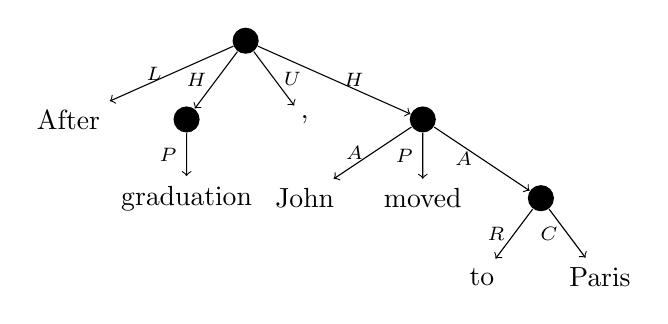
\begin{tikzpicture}[level distance=10mm, ->]
    \node (ROOT) [fill=black, circle] {}
      child {node (After) {After} edge from parent node[left] {\scriptsize $L$}}
      child {node (graduation) [fill=black, circle] {}
      {
        child {node {graduation} edge from parent node[left] {\scriptsize $P$}}
      } edge from parent node[left] {\scriptsize $H$} }
      child {node {,} edge from parent node[right] {\scriptsize $U$}}
      child {node (moved) [fill=black, circle] {}
      {
        child {node (John) {John} edge from parent node[left] {\scriptsize $A$}}
        child {node {moved} edge from parent node[left] {\scriptsize $P$}}
        child {node [fill=black, circle] {}
        {
          child {node {to} edge from parent node[left] {\scriptsize $R$}}
          child {node {Paris} edge from parent node[left] {\scriptsize $C$}}
        } edge from parent node[left] {\scriptsize $A$} }
      } edge from parent node[right] {\scriptsize $H$} }
      ;
  \end{tikzpicture}
\end{figure*}

The corresponding dependency tree is given in the following figure:

\begin{figure*}[h]
\centering
\begin{dependency}[theme = simple]
\begin{deptext}[column sep=.7em,ampersand replacement=\^]
After \^ graduation \^ , \^ John \^ moved \^ to \^ Paris \\
\end{deptext}
\depedge{2}{1}{L}
\depedge{2}{3}{U}
\depedge{5}{4}{A}
\depedge{2}{5}{H}
\depedge{7}{6}{R}
\depedge{5}{7}{A}
\end{dependency}
\end{figure*}

\section{Additional UCCA-annotated examples}

\paragraph{Linkage.}

The following figure demonstrates a linkage relation, omitted from Figure 1a in the paper.

\begin{figure}[H]
  \centering
  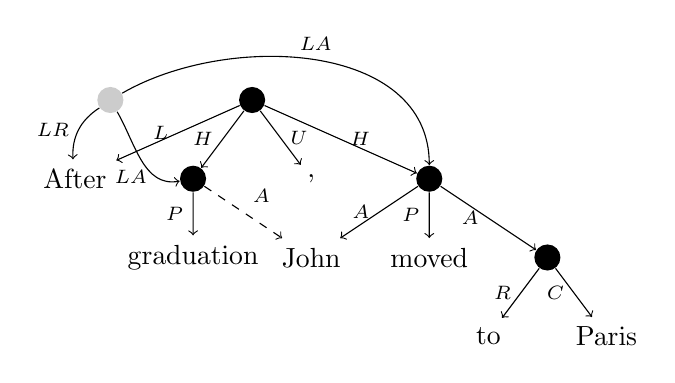
\begin{tikzpicture}[level distance=10mm, ->]
    \node (ROOT) [fill=black, circle] {}
      child {node (After) {After} edge from parent node[left] {\scriptsize $L$}}
      child {node (graduation) [fill=black, circle] {}
      {
        child {node {graduation} edge from parent node[left] {\scriptsize $P$}}
      } edge from parent node[left] {\scriptsize $H$} }
      child {node {,} edge from parent node[right] {\scriptsize $U$}}
      child {node (moved) [fill=black, circle] {}
      {
        child {node (John) {John} edge from parent node[left] {\scriptsize $A$}}
        child {node {moved} edge from parent node[left] {\scriptsize $P$}}
        child {node [fill=black, circle] {}
        {
          child {node {to} edge from parent node[left] {\scriptsize $R$}}
          child {node {Paris} edge from parent node[left] {\scriptsize $C$}}
        } edge from parent node[left] {\scriptsize $A$} }
      } edge from parent node[right] {\scriptsize $H$} }
      ;
    \draw[dashed,->] (graduation) to node [auto] {\scriptsize $A$} (John);
    \node (LKG) at (-1.8,0) [fill=black!20, circle] {};
          \draw[bend right] (LKG) to node [auto, left] {\scriptsize $LR$} (After);
          \draw (LKG) to[out=-60, in=190] node [below] {\scriptsize $LA\quad$} (graduation);
          \draw (LKG) to[out=30, in=90] node [above] {\scriptsize $LA$} (moved);
  \end{tikzpicture}
\end{figure}

\paragraph{Longer example.}

The following figure shows the UCCA annotation for the sentence
``A similar technique is almost impossible to apply to other crops, such as cotton, soybeans and rice.''.
The sentence was used by \cite{oepen2015semeval} to compare between the difference schemes.
It includes a single Scene, whose main relation is ``apply'', a secondary relation ``almost impossible'', as well as two complex arguments: ``a similar technique'' and the coordinated argument ``such as cotton, soybeans, and rice.''

\begin{figure}[H]
  \centering
  \scalebox{.6}{
  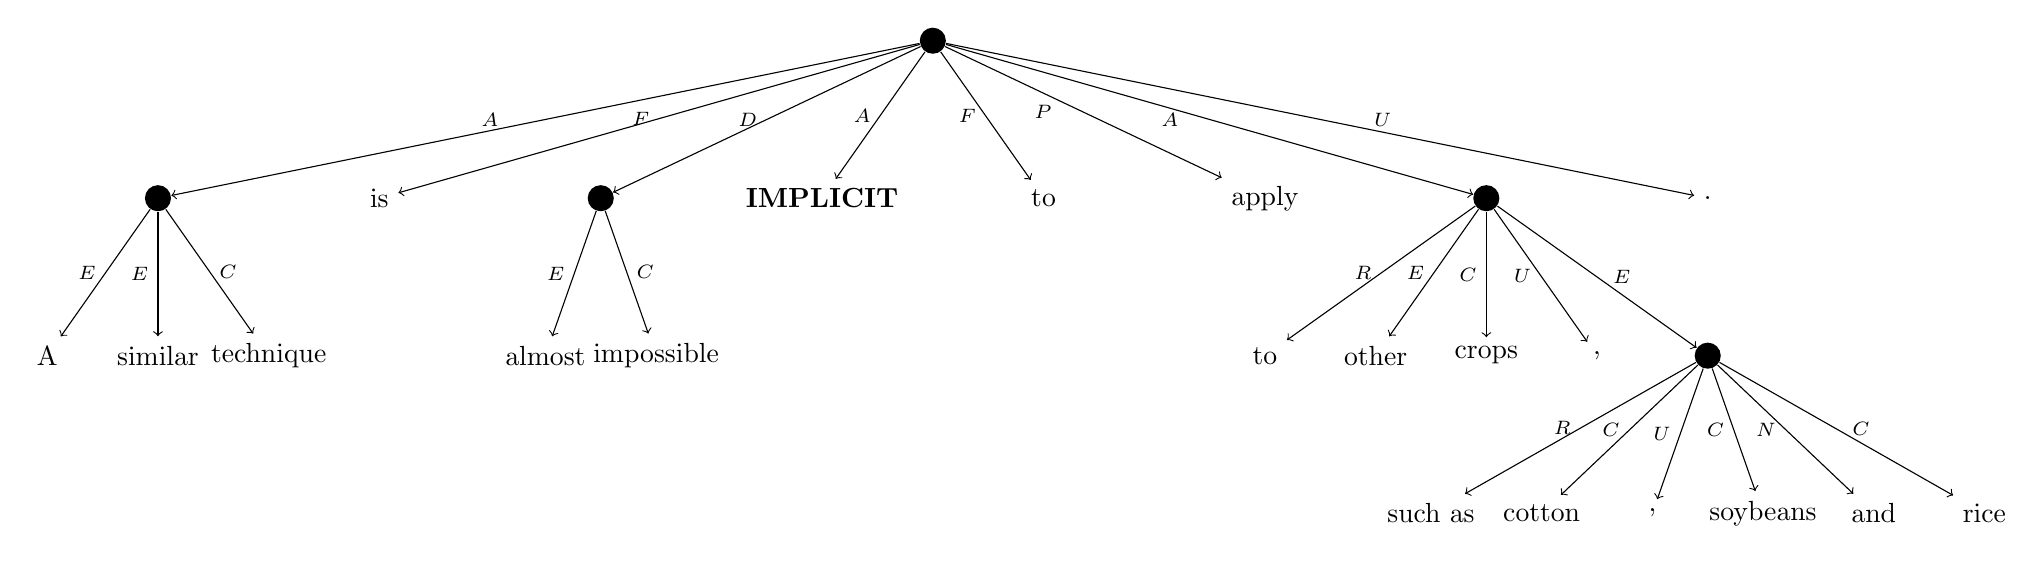
\begin{tikzpicture}[level distance=20mm, ->,
  level 1/.style={sibling distance=8em},
  level 2/.style={sibling distance=4em},
  level 3/.style={sibling distance=4em}]
    \node (ROOT) [fill=black, circle] {}
      child {node [fill=black, circle] {}
      {
        child {node {A} edge from parent node[left] {\scriptsize $E$}}
        child {node {similar} edge from parent node[left] {\scriptsize $E$}}
        child {node {technique} edge from parent node[right] {\scriptsize $C$}}
      } edge from parent node[left] {\scriptsize $A\quad$ \hspace{1mm} } }
      child {node {is} edge from parent node[left] {\scriptsize $F$}}
      child {node [fill=black, circle] {}
      {
        child {node {almost} edge from parent node[left] {\scriptsize $E$}}
        child {node {impossible} edge from parent node[right] {\scriptsize $C$}}
      } edge from parent node[left] {\scriptsize $D$} }
      child {node {\textbf{IMPLICIT}} edge from parent node[left] {\scriptsize $A$}}
      child {node {to} edge from parent node[left] {\scriptsize $F$}}
      child {node {apply} edge from parent node[left] {\scriptsize $P\quad$}}
      child {node [fill=black, circle] {}
      {
        child {node {to} edge from parent node[left] {\scriptsize $R$}}
        child {node {other} edge from parent node[left] {\scriptsize $E$}}
        child {node {crops} edge from parent node[left] {\scriptsize $C$}}
        child {node {,} edge from parent node[left] {\scriptsize $U$}}
        child {node [fill=black, circle] {}
        {
          child {node {such as} edge from parent node[left] {\scriptsize $R$}}
          child {node {cotton} edge from parent node[left] {\scriptsize $C$}}
          child {node {,} edge from parent node[left] {\scriptsize $U$}}
          child {node {soybeans} edge from parent node[left] {\scriptsize $C$}}
          child {node {and} edge from parent node[left] {\scriptsize $N$}}
          child {node {rice} edge from parent node[right] {\scriptsize $\; C$}}
        } edge from parent node[right] {\scriptsize $\; E$ \hspace{1mm} } }
      } edge from parent node[left] {\scriptsize $A\;$ \hspace{1mm} } }
      child {node {.} edge from parent node[right] {\scriptsize $\quad \quad U$}}
      ;
  \end{tikzpicture}
  }
\end{figure}



\bibliography{references}
\bibliographystyle{acl2016}

\end{document}